%% Anfroderungen.tex
%% $Id: Anfroderungen.tex 28 2007-01-18 16:31:32Z bless $

Die Aufgabenstellung bestand darin, herauszufinden, ob ein personalisiertes Vibrationsmuster besser als ein vorgegebenes Vibrationsmuster erkannt wird.
Die Grundvorraussetzung sollte ein System sein, dass mit dem Wearable kommuniziert und Daten {\"u}bertragen kann, so dass das Wearable Vibrationen abspielt. 
Dar{\"u}ber hinaus soll eine Studie erstellt werden, in der man herausfindet, ob es einen signifikanten Unterschied zwischen generischen und genetischen Vibrationen gibt. 
Die generischen Vibrationen sind fest vorgegeben, wobei die genetischen Vibrationen, anhand der Bewertungen des Probanden angepasst werden sollen. 
Dabei habe man ein Evolution{\"a}ren Algorithmus verwendet um die genetischen Werte f{\"u}r einen Probanden zu bestimmen. 

Zunächst musste man sich im Vorfeld ein paar Gedanken {\"u}ber die Repr{\"a}senatation eines Signals, die Dekodierung und die {\"U}bertragung machen.
%Um dies zu l{\"o}sen musste man sich im Vorfeld ein paar Gedanken {\"u}ber die Repr{\"a}senatation eines Signals, um die Dekodierung und {\"u}ber die {\"U}bertragung machen.
Im Folgenden werden diese Entscheidungsfindungen beschrieben.

\paragraph{Wearable}

\begin{figure}
	\centering
    \includegraphics[width=\textwidth]{pics/wristband111.jpg}
    \caption{Armband ge{\"o}ffnet. Komponenten 2 Traktoren, Batterie, und Mikroprozessor}
    \label{fig:wristband1}
\end{figure}

\begin{figure}
	\centering
    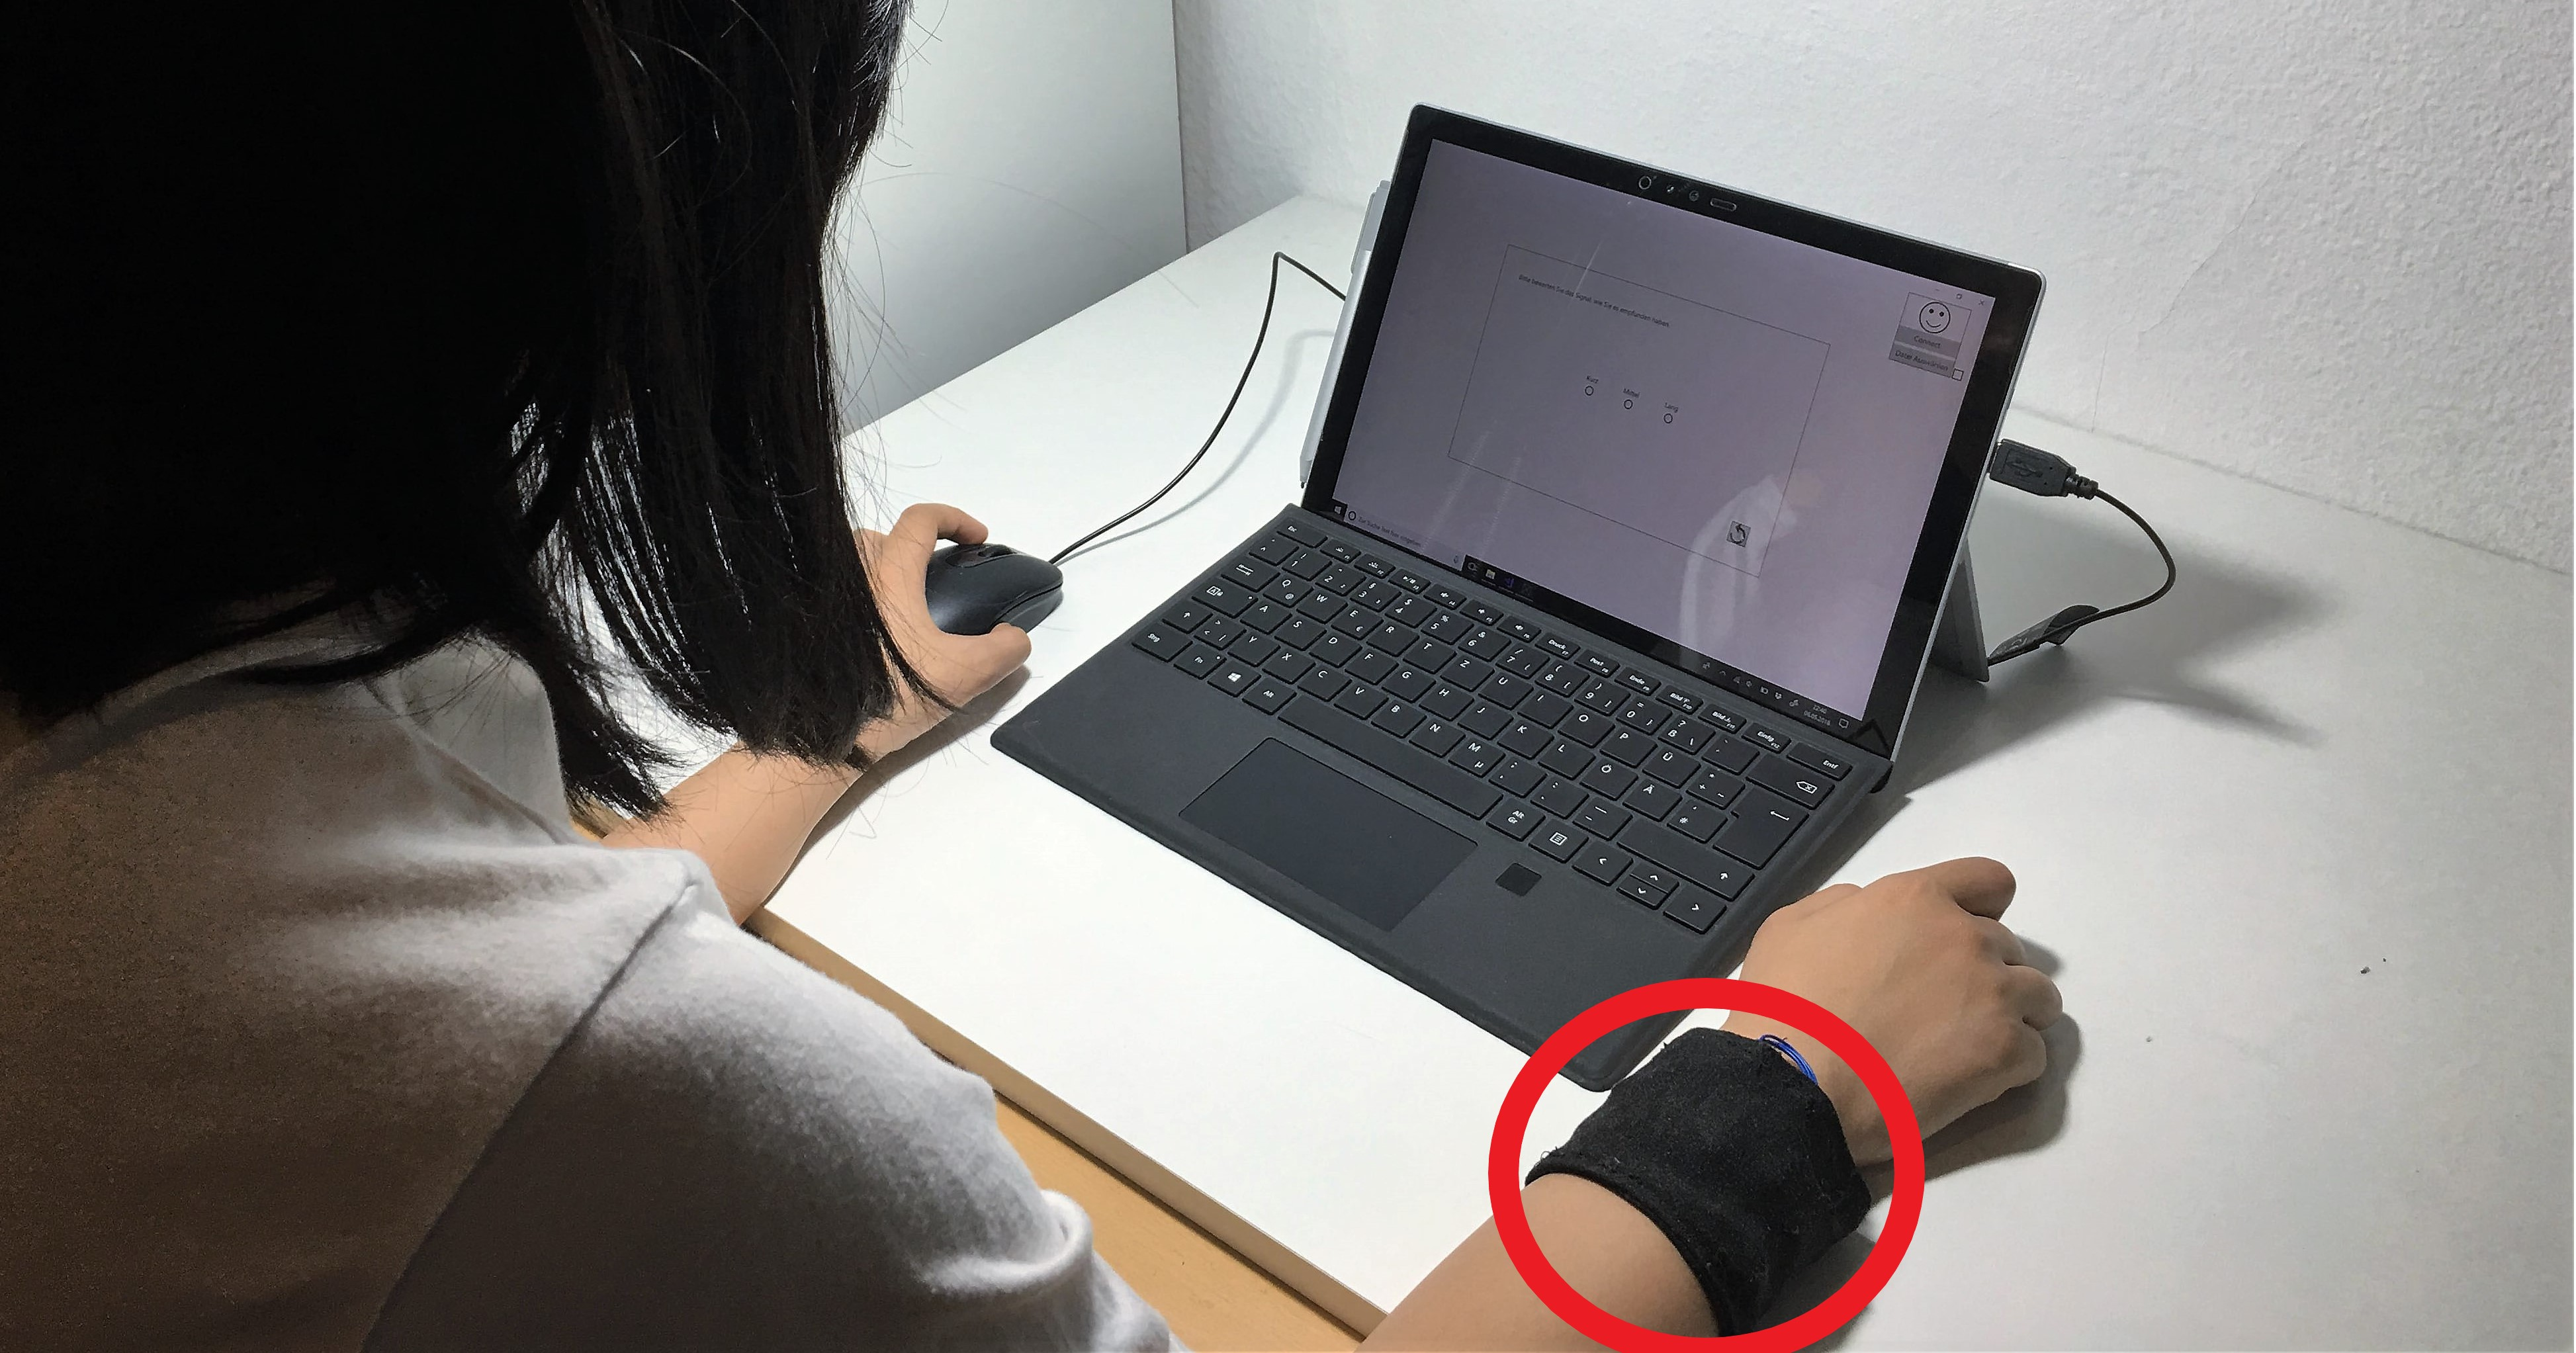
\includegraphics[width=\textwidth]{pics/peter.png}
    \caption{Armband angezogen}
    \label{fig:wristband2}
\end{figure}

Damit man Vibrationen {\"u}berhaupt darstellen kann, h{\"a}tte man sich ein eigenes Taktiles Device entwerfen m{\"u}ssen. In meinem Fall war dies nicht n{\"o}tig, da das Wearable vom TECO vorgegeben war. Zu den Komponenten des Wearables gehören zwei Taktoren (TI TLC5971), einen Mikroprozessor (nRF51822 / BLE Nano) und eine Batterie.

Die Kommunikation des Armbands konnte man {\"u}ber eine Serielle Schnittstelle, sowie {\"u}ber Bluetooth Low Energie (LE) realisieren.
Bei der seriellen Schnittstelle ist ein USB-Kabel n{\"o}tig gewesen um den PC mit dem Wearable anzusprechen, dabei w{\"a}re die Mobilit{\"a}t verloren gegangen. Daher habe man die verf{\"u}gbare BLE Schnittstelle benutzt um zwischen dem PC und dem Wearable zu kommunizieren. 

Bluetooth LE {\"u}bertr{\"a}gt Nachrichten nur in einer maximalen Gr{\"o}{\ss}e von 20 Bytes. Diese werden jeweils als zwei Bytes Bl{\"o}cke {\"u}bertragen. 

Anhand der Begrenzung der Daten{\"u}bertragung hat man sich eine geeignete Dekodierung des Signals {\"u}berlegen m{\"u}ssen. 

Die Programmiersprache um die Kommunikation zwischen dem PC und dem Wearable aufzubauen, konnte frei gew{\"a}hlt werden. 
Dafür habe man zuvor verschiedenste Programmiersprachen untersucht. 
Java hat man nach fehlenden Informationen zum Kommunikationsaufbau ausgeschlossen.
%Java hat man nach fehlenden Informationen zum Kommunikationsaufbau ausgeschlossen. 
Schlie{\ss}lich hat man sich f{\"u}r C\# entschieden, da hier ausf{\"u}hrliche Dokumentationen vorhanden waren.
%Die weiteren Gründe waren ebenfalls ausschlaggebend, für die Wahl der Programmiersprache und zwar eine erfolgreiche 
%Dadurch, dass man eine funktionierende Kommunikation realisiert hatte, eine einfache Grafische Benutzeroberfl{\"a}che hinzufügen konnte die für die sp{\"a}tere Studie hilfreich sein konnte, waren die anderen Gründe um sich für die Programmiersprache  zu entscheiden.
Außerdem hat man sich für diese Programmiersprache wegen ihrer funktionsfähigen Kommunikation und der einfachen Grafischen Benutzeroberfl{\"a}che entschieden. 
Die Grafische Benutzeroberfl{\"a}che hat man für die Studie verwendet.
% Nach einer erfolgreich funktionierenden Kommunikation hat und man gleichzeitig eine Grafische Benutzeroberfl{\"a}che nutzen konnte, die f{\"u}r die sp{\"a}tere Studie hilfreich sein k{\"o}nnte.
%eine funktionierende Kommunikation aufgebaut hat und man gleichzeitig die Grafische Benutzeroberfl{\"a}che nutzen kann um Studie darin durchzuf{\"u}hren. 

Dabei musste herausfinden was f{\"u}r Einstellungsm{\"o}glichkeiten das Wearable besitzt. Diese waren die L{\"a}nge und die St{\"a}rke eines Signals.

\paragraph{Signale}

Ein Signal repr{\"a}sentiert eine Vibration, die auf dem Wearable abgespielt wird. Es hat sich die Frage gestellt, wie personalisiert man denn jetzt Signale. Hier hat man das Signal in drei verschiedene L{\"a}ngen definiert, \textbf{Kurz}, \textbf{Mittel} und \textbf{Lang}. 

Dabei hatte man als Vorgabe, dass man einen Evolution{\"a}ren Algorithmus (EA) benutzen sollte.
Diesen EA hat man verwendet, um f{\"u}r die Signaltypen ein personalisierten Wert zu bestimmen.

Man hat sich ein Vorgang {\"u}berlegen m{\"u}ssen, um f{\"u}r den EA eine Startpopulation zu erzeugen; die Individuen der Population zu bewerten; mittels einer Fitnessfunktion den Fitnesswert f{\"u}r jedes Individuum zu berechnen; eine geeignete Selektion, Reproduktion und Mutation, sowie die Terminierungsbedingung zu bestimmen. 

Eine geeignete Signalrepr{\"a}sentation musste definiert werden um Signale vom PC zum Wearable {\"u}ber BLE zu senden und abspielen zu lassen. Das bedeutet sowohl am PC als auch am Wearable selbst musste dies definiert werden.

\paragraph{Studie}

Es sollte eine Grafische Benutzeroberfl{\"a}che erstellt werden, damit der Proband die Studie komplett {\"u}ber das Programm ausf{\"u}hren kann, indem er die Instruktionen des Programms folgt.

Es hat sich durch das Definieren der Signale und dem EA ergeben, dass die Studie in drei Schritten unterteilt wird. 
In dem ersten Schritt muss man Grenzen f{\"u}r die Erzeugung einer Startpopulation f{\"u}r einen EA bestimmen.
%Der erste Schritt ist es, die Grenzen f{\"u}r eine Startpopulation f{\"u}r einen EA zu bestimmen. 
Der zweite Schritt ist es, einen genetischen Wert f{\"u}r die eigentliche Studie zu bestimmen, dies passiert durch ausf{\"u}hren mehrerer Generationen des EA. 
Als letzen Schritt definiert man eine Folge von generischen und genetischen Signalen, die man anschlie{\ss}end vom Benutzer bewerten l{\"a}sst.
%Schlie{\ss}lich ist der letzte Schritt, dass man sich eine Folge von generische und genetische Signalen definiert, die man anschlie{\ss}end vom Benutzer bewerten zu l{\"a}sst.
%Der letzte Schritt ist es, generische und genetische Signale vom Benutzer bewerten zu lassen.

Alle Daten sollten {\"u}berpr{\"u}ft werden und es sollte herausgefunden werden, ob es am signifikante Unterschiede gibt.



%Zu aller erst hat man sich das vorgegebene Armband genauer inspiziert. Dabei konnte man das Armband {\"u}ber eine Serielle Schnittstelle sowie {\"u}ber Bluetooth Low Energie (LE) nutzen. 
%Bei der Nutzung der Seriellen Schnittstelle hatte man zwar den Vorteil, dass man sich nicht mittels Bluetooth auseinander setzen m{\"u}sse, jedoch ist man an einem Kabel {\"u}ber den PC verbunden gewesen, was zur Einschr{\"a}nkung der Bewegungsfreiheit \dots hat. 
%Um genau diesen Nachteil nicht zu haben hat man sich f{\"u}r Bluetooth LE entschieden. 
%Dabei gab es auch einige Nachteile, die man beheben musste. Die Kommunikation mittels Bluetooth LE hatte eine maximale Daten{\"a}bertragung von 20 Bytes. Diese wurden jeweils in zwei Bytes Bl{\"o}cke unterteilt.

%Anhand der Begrenzung der Daten{\"u}bertragung hat man sich eine geeignete Dekodierung des Signals {\"u}berlegen m{\"u}ssen. 











%\dots
%Dabei musste man sich definieren wie ein Signal aufgebaut gewesen ist. Dabei musste f{\"u}r ein Signal eine Datenstruktur erstellt werden. 



%Dekodierung eines Signals.

%Evolution{\"a}rer Algorithmus musste erstellt werden mit allen komponenten, Population Fitness funktion, usw

%Kommunikation mit dem Armband musste aufgebaut werden. 

%Es sollte eine Studie ausgef{\"u}hrt werden um das System zu testen 

%Dabei sollte eine Grafische Oberfl{\"a}che erstellt werden, damit der Benutzer selbst eine Eingabe in den PC machen konnte um n{\"a}chste Signale abspielen zu k{\"o}nnen.

%Es sollten die Daten ausgewertet werden.
